\section{Elektronowa teoria materii}
\subsection{Początki teorii elektronowej (subiektywnie)}
\begin{table}[h!]
    \centering
    \begin{tabular}{ll|ll|ll}
        \multicolumn{2}{c}{Elektrodynamika} & 
		\multicolumn{2}{|c|}{Teoria kinetyczna} & 
		\multicolumn{2}{c}{Teoria kwantowa} \\
            &&   1803 r. J. Dalton: & atomy   &&     \\
        1822 r. H. Davy: & $\sigma \sim S/L$ &&    &&     \\
        1826 r. G. Ohm: & $I \sim V$         & 1827 r. R. Brown: & ruchy  && \\
        1845 r. G. Kirchhoff: & $ j \sim E_f$& &&& \\
        1861 r. J. Maxwell: & równania & 1860 r. J. Maxwell: & rozkład $v$ && \\
        && 1865 r. J. Loschmidt: & rozmiar at. && \\
        && 1867 r. J. Maxwell: & równanie && \\
        && \multicolumn{2}{r|}{ciągłości o strukturze r. kinet.} && \\
        && 1872 r. L. Boltzmann: & równanie && \\
        1881 r. Helmholtz: & \multirow{2}{*}{elektron} &&&&\\
        Johnstone Stoney: &  &&&& \\
        1897 r. J. J. Thompson && 1900 r. D. Hilbert && 1900 r. M. Planck & \\
	&& 1905 r. Einstein i  & teoria r. && \\
	&& Smoluchowski: & Browna && \\ 
	1908 r. R. Millikan:& wart. $e$ &&&& \\ 
	1910 r. E. Rutherford:& budowa at. &&&&\\
	&& 1913 r. Bohr:& model at. && \\
	1916 r. Tolman-Steward:& bezwł. el. &&&&\\
	&&&& 1924 r. L. de Broglie & \\
	&&&& 1926 r. E. Schr\"{o}dinger & \\
	&&&& 1927 r. Fermi i Dirac: & stat. kw. \\
    \end{tabular}
\end{table}
Elektronowa teoria meterii 
\begin{itemize}
	\item[1845 r.] G. Fechner - Model prądu elektronowego 
	\item[1846 r.] W. Weber - Elektrodynamika cząstek
		$$ F = \dfrac{q_1q_2}{r^2} \left\{ 1 + \dfrac{r}{c^2} \ddot{r} (t) -
		\dfrac{1}{2c^2} \left[ \dot{r} (t) \right]^2 \right\} $$
	\item[1881 r.] Helmholtz
	\item[1897 r.] H. A. Lorentz - teoria elektronowa
	\item[1898 r.] E. Riecke - 
	\item[1900 r.] Drude - model przewodnictwa
	\item[1927 r.] Sommerfeld A. - statystyki kwantowe do opisu elektronów
	\item[1928 r.] Block
\end{itemize}
Teorie na przestrzeni czasu:
\begin{itemize}
	\item[1900 $\div$ 1927] Klasyczna teoria transportu elektronowego 
	\item[1927 $\div$ 1928] Półklasyczna teoria transportu elektronowego
	\item[1928 $\div$ 1933] Współczesna teoria transportu elektronowego 
\end{itemize}

%%%%%%%%%%%%%%%%%%%%%%%%%%%%%%%%%%%%%%%%%%%%%%%%%%%%%%%%%%%%%%%%%%%%%%%%%%%%%%%%%%
% new subsubsection
%%%%%%%%%%%%%%%%%%%%%%%%%%%%%%%%%%%%%%%%%%%%%%%%%%%%%%%%%%%%%%%%%%%%%%%%%%%%%%%%%%
\subsection{Teoria elektronowa Lorenza}
\textbf{Założenia:}
\begin{enumerate}
	\item Ośrodki materiale mają strukturę dyskretną, tzn. zbudowane są z 
		cząstek naładowanych, które w sumie dają układ neutralny.
	\item Wszystkie zjawiska w ośrodku materialnym są spowodowane ruchem 
		cząstek naładowanych pod wpływem pól zewnętrznych, przy czym:
		\begin{enumerate}
			\item w dielektrykach cząstki naładowane są związane i mogą
				wykonywać drgania wokół położeń równowagi lub ulegać
				nieznacznym wychyeniom pod wpływem przyłożonego $\vec{E}$,
			\item w przewodnikach prócz cząstek związanych występują także
				czastki naładowane swobodne, których ruch powoduje 
				powstanie prądu elektrycznego,
			\item w ośrodkach magnetycznych istnieją cząstki naładowane 
				posiadające wewnętrzny moment magnetyczny lub niezerowy
				moment pędu.
		\end{enumerate}
	\item Mikroskopowe pola elektromagnetyczne wytwarzane przez cząstki 
		naładowane tworzące rozpatrywany ośrodek są rozwiązaniami 
		równań Maxwella w próżni:\\
	\begin{equation}{\label{Max_mikro}}
	\left\{ 
		\begin{array}{l}
		\nabla \circ \vec{e} (\vec{r},t) = \rho(\vec{r},t)\\
		\nabla \times \vec{b}(\vec{r},t) - \partial_t \vec{e}(\vec{r},t) 
			= \vec{j}(\vec{r},t)\\
		\nabla \times \vec{e} (\vec{r},t) + \partial_t \vec{b} (\vec{r},t)
			= \vec{0} \\
		\nabla \circ \vec{b} (\vec{r},t) = 0.
		\end{array}
	\right.
	\end{equation}
	$\vec{e}(\vec{r},t), \ \vec{b}(\vec{r},t)$  - mikroskopowe pola elektryczne i
		magnetyczne \\
	$\rho (\vec{r},t)= \sum_i q_i \delta (\vec{r} -  \vec{r_i} (t))$\\
	$\vec{j}(\vec{r},t)= \sum_i \vec{v_i} (t) \delta(\vec{r} - \vec{r_i}(t))$
	\item Gęstość siły działająca na $\vec{\rho}(\vec{r},t)$ ma postać
	$$ \vec{f}(\vec{r},t) = \vec{\rho}(\vec{r},t) [ \vec{e}(\vec{r},t)+ \vec{v}(t)
		\times \vec{b}(\vec{r},t)] $$
	$$ \vec{F} (t) = \int d^3r' f(\vec{r}\ ',t) = $$
	przy założeniu jednorodności $\vec{b}$ i $\vec{e}$
	$$ = \int d^3r' \{ \rho \arg [ \vec{e} + \vec{v}(t) \times \vec{b} ]  \} =
	\int d^3r' \{ q \delta (\vec{r} - \vec{r}\ ') [ \vec{e} + \vec{v}(t) 
	\times \vec{b} ] \} = q[ \vec{e} + \vec{v}(t) \times \vec{b} ] \int d^3r' 
	\delta (\vec{r} - \vec{r} \ ').$$
	Ostatecznie
	\begin{equation}
		\vec{F} = q (\vec{e} + \vec{v} \times \vec{b})
	\end{equation}
	\begin{equation}
		m\ddot{\vec{r}} (t) = q[ \vec{e} + \vec{v} (t) \times \vec{b} ]. 
	\end{equation}
\end{enumerate}
Zmiany przestrzenne $\vec{e} \arg$ i $\vec{b} \arg $ są znaczące na odcinkach
rzędu $10^{-10} \mbox{m} = 1 \stackrel{\circ}{\mbox{A}} = 0,1 \mbox{nm}.$\\
Zmiany czasowe są rzędu $10^{-13} \div 10^{-17}$s. 
\\
Klasyczny promień elektronu $r_e = \frac{1}{4\pi \epsilon_0} \frac{e^2}{mc^2} 
\approx 2,82 \cdot 10^{-6}$nm, rozmiar protonu $r_p \approx 0,88 \cdot 
10^{-6}$nm natomiast promień atomu $r_p \approx 0,1$nm.

%%%%%%%%%%%%%%%%%%%%%%%%%%%%%%%%%%%%%%%%%%%%%%%%%%%%%%%%%%%%%%%%%%%%%%%%%%%%%%%%%%
% new subsection
%%%%%%%%%%%%%%%%%%%%%%%%%%%%%%%%%%%%%%%%%%%%%%%%%%%%%%%%%%%%%%%%%%%%%%%%%%%%%%%%%%
\subsection{Makroskopowa elektrodynamika ośrodków materialnych}
\textbf{Hipotezia: }
Makroskopowe pola $\vec{E}$ i $\vec{B}$ są wartościami średnimi pól 
mikroskopowych$\vec{e}$ i $\vec{b}$.
\begin{equation}
	\vec{E} \arg = \left< \vec{e} \arg \right>
\end{equation}
\begin{equation}
	\vec{B} \arg = \left< \vec{b} \arg \right>,
\end{equation}
gdzie średnia jest przestrzenna, czyli
$$ \left< \vec{f} \arg \right> \equiv \int d^3 r' w(\vec{r}\ ')\vec{f}
( \vec{r} - \vec{r}\ ',t). $$
$w(\vec{r}\ ')$ - funkcja wagowa spełniająca warunki:
\begin{enumerate}
	\item jest funkcją rzeczywistą dodatnio określoną,
	\item jest znormalizowana $$\int_{\Omega} d^3 r' w(\vec{r}\ ') = 1,$$
	\item jest wolnozmienna, tj.
		$$w(\vec{r}\ '+\vec{a}) = \sum_n \frac{1}{n!} \left[ \vec{a} \nabla 
		\right]^n w(\vec{r})_{\big|_{\vec{r}=\vec{r}'}}$$
		$$w(\vec{r}\ '+\vec{a}) = w(\vec{r}\ ')\pm[\vec{a}\nabla] 
		w(\vec{r}\ ') +\frac{1}{2} [\vec{a}\nabla]^2w(\vec{r}\ '),$$
	\item rozciągłość duża w porównaniu z wielkością cząstek.
\end{enumerate}
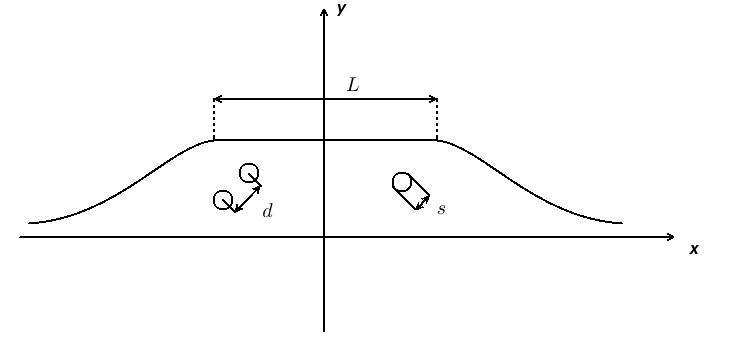
\includegraphics[scale=1]{W1_struktura_2.png}
$$L \sim 10\div 100 \mbox{ nm}$$
$$s\sim 10^{-5} \mbox{ nm}$$
$$d \sim 0,1 \mbox{ nm}$$
\subsubsection{Wyprowadzenie makroskopowych praw Maxwella z 
mikroskopowych odpowiedników}
Zgodnie z równaniami mikroskopowymi \ref{Max_mikro}:
\begin{equation} 
	\nabla \cdot \vec{E}\arg=\left< \rho \arg \right> \label{startr1}
\end{equation}
\begin{equation} 
	\nabla \times \vec{B}\arg-\partial_t\vec{E}\arg=\left< \vec{j}\arg
	\right> \label{startr2}
\end{equation}
\begin{equation} 
	\nabla \times \E+\partial_t \B=\vec{0} \label{startr3}
\end{equation}
\begin{equation} 
	\nabla \cdot \B=0 \label{startr4}
\end{equation}
\begin{center}
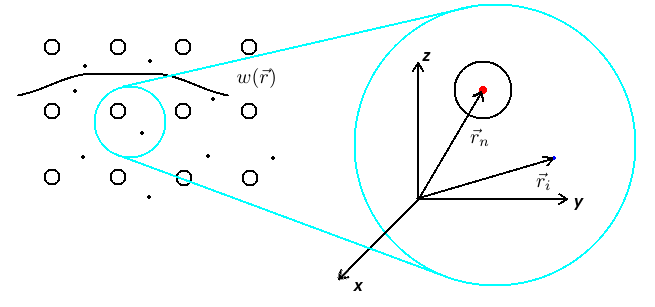
\includegraphics[scale=0.8]{W1_struktura_3.png}
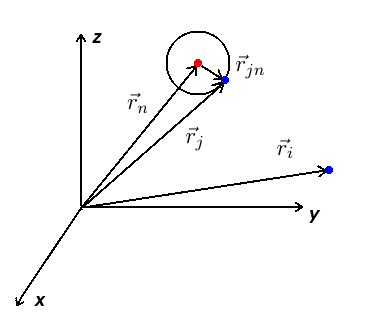
\includegraphics[scale=0.8]{W1_struktura.png}
\end{center}
Najpierw obliczymy średnią z gęstości ładunków.
Gęstość ładunku można rozbić na gęstość ładunków swobodnych oraz 
gęstość ładunków związanych
$$\rho \arg = \rho_{free} \arg + \rho_{bound} \arg$$
gdzie:\\
$\rho_{free} \arg = q_e \sum\limits_i \delta (\vec{r}-\vec{r}_i(t))$\\
$\rho_{bound} \arg = \sum\limits_n \underbrace{\rho_n\arg}_{n-tego\
jonu}  = \sum\limits_n \sum\limits_j q_{jn} \delta (\vec{r}-\vec{r}_j(t)) 
= \sum\limits_{n} \sum\limits_{j} g_{jn}\delta(\vec{r}-\vec{r}_n(t)-
\vec{r}_{jn}(t)).$\\
$$\ave{ \rho \arg } = \ave{\rho_{free}\arg} + \ave{\rho_{bound}\arg} = $$
$=\int d^3r' w(\vec{r}\ ') \rho_{free}(\vec{r}-\vec{r}_j\ '(t))+
\int d^3r' w(\vec{r}\ ') \rho_{bound}(\vec{r}-\vec{r}_j\ '(t))=$\\
$ = \int d^3r' w(\vec{r}\ ')q_e \sum\limits_{i}\delta (\vec{r}-\vec{r}_i(t)
-\vec{r}\ ') + \int d^3r' w(\vec{r}\ ') \sum\limits_n \sum\limits_j q_{jn}
\delta (\vec{r}-\vec{r}_j\ '(t) - \vec{r}\ ')= $\\
$ = q_e \sum\limits_i w(\vec{r} - \vec{r}_i(t)+ \sum\limits_n \sum\limits_j q_{in} 
w(\vec{r}-\vec{r}_n(t)-\vec{r}_{jn}(t)=(*) .$
Z własności $w$ wiemy, że:
$$w(\vec{r}-\vec{r}_n(t)-\vec{r}_{jn}(t))\simeq w(\r-\r_n(t))-
[\r_{jn}\cdot\nabla]w(\r-\r_n(t)).$$
$(*)=  q_e \sum\limits_i w(\vec{r} - \vec{r}_i(t))+ \sum\limits_n 
\sum\limits_j q_{in} 
[w(\r-\r_n(t))-[\r_{jn}\cdot\nabla]w(\r-\r_n(t))]$\\
Całkowity ładunek jonu: $q_n=\sum\limits_j q_{jn}$.\\
Moment dipolowy $\vec{d}_n(t)=\sum\limits_j d_{jn}(t) = 
\sum\limits_j q_{jn}\vec{r}_{jn}(t).$\\
$$\ave{ \rho \arg } = q_e\sum_i w(\r-\r_i(t))+\sum_n q_n w(\r-\r_n(t))-\nabla\cdot
\sum_nw(\r-\r_n(t))\vec{d}_n$$
$$\ave{ \rho \arg } =\underbrace{\ave{ q_e\sum_i \delta(\r-\r_i(t))}+\ave{\sum_n q_n 
\delta(\r-\r_n(t))}}_{\mbox{makroskopowa gęstość ładunku}}-\nabla\cdot
\underbrace{\ave{\sum_n\delta(\r-\r_n(t))\vec{d}_n(t)}}_{\mbox{makroskopowa
polaryzacja}}$$
$$\ave{\rho\arg}=\Brho\arg - \nabla\cdot\vec{P}\arg.$$
Wracając do równania \ref{startr1}
$$\nabla\cdot\vec{E}\arg=\ave{\rho\arg}=\Brho\arg-\nabla\vec{P}\arg$$
$$\nabla\cdot(\vec{E}\arg+\nabla\vec{P}\arg)=\Brho\arg$$
$$ \vec{E}\arg+\nabla\vec{P}\arg\equiv\vec{D}\arg$$
gdzie $\vec{D}\arg$ - wektor indukcji elektrycznej
$$D_i\arg=\sum_{k/1}^{3}\int d^3r\int_{-\infty}^{t}dt'\epsilon_{kj}(\vec{r},
\vec{r}\ ',t,t')E_j(\vec{r}\ ',t')$$
$$D_i=\sum_{k/1}^3\epsilon_{kj}E_j.$$
